\vspace{-2mm}
\section{Recommendation}
\label{Recommendation}
We show in this section how to leverage our \graphsim metric to generate artificial (AlterEgo) profiles of users in domains where the users might not have any activity yet. We present both a privacy-preserving (\crossrec) and a non-privacy-preserving (\npcrossrec) schemes.\footnote{Recall that \npcrossrec is used to demonstrate the effectiveness of \graphsim without the additional privacy overhead.}  
% the recommendation computation scheme underlying both our \crossrec (as well as \npcrossrec\footnote{We denote a non-private version of \crossrec as \npcrossrec.}) which consists of the following four phases.

\subsection{Similarity Computation Phase}
We call the similarities computed in this phase as the \emph{baseline} similarities. For this phase, \crossrec treats both the source and target domains as a single domain and computes all pairwise item similarities. Basically, \crossrec computes the adjusted cosine similarities between the items in $I^S \cup I^T$ based on the preferences of the users in $U^S \cup U^T$ for these items. We distinguish two types of similarities which are as follows.

\noindent{\bf Homogeneous similarities.} These similarities are computed between items in the same domain. For instance, the similarity between a book and another one is homogeneous. Such similarities are used for intra-domain extension in \autoref{Implementation}.

\noindent{\bf Heterogeneous similarities.} These similarities are computed between items in different domains. For instance, the similarity between a book and a movie is heterogeneous. Such similarities are used for cross-domain extension in \autoref{Implementation}.

This phase remains the same for both \crossrec as well as \npcrossrec.


\subsection{X-Sim Computation Phase}
After the computation of the baseline item-item similarities, \crossrec uses the \graphsim metric at first within a single domain to extend and improve the connections between the bridge items of a domain and other items within the same domain. \crossrec uses the \graphsim metric to extend the similarities between items across the domains (which we explain in more details in~\autoref{Implementation}). At the completion of the heterogeneous similarity extension, for each item in source domain ($D^S$), there exists a corresponding set of items in target domain ($D^T$) with quantified (positive or negative) \graphsim values. This phase is the same for both \crossrec as well as \npcrossrec.

\subsection{AlterEgo Generation Phase}
In this phase, the profile of Alice (in $D^S$) is mapped to her AlterEgo profile (in $D^T$) as shown in Figure~\ref{fig:alterego}. For pedagogical reasons, we first present the non-private case followed by the private one.

%\subsubsection*{{\it \large\npcrossrec} AlterEgo generation}
\noindent{\bf \npcrossrec AlterEgo generation.} The non-private mapping is performed in two step which are as follows.

{\it Similar item computation.} In this step, for every item $i$ in $D^S$, we determine the replacement item $j$ in $D^T$. Here, $j$ is the item which is most similar to $i$ based on the heterogeneous similarity computed using \graphsim.


{\it AlterEgo profile construction.} We then replace every item rated by Alice in $D^S$ with the most similar item in $D^T$ computed in the previous step. This item replacement induces the AlterEgo profile\footnote{If Alice has rated a few items in $D^T$ then the mapped profile is appended to her original profile in $D^T$ to build her AlterEgo profile.} of Alice in the target domain as shown in Figure~\ref{fig:alterego}.\\
This AlterEgo profile of Alice is the mapped profile of Alice from the source domain to the target domain.
\begin{figure}[!htb]
\begin{center}
\vspace{-7mm}
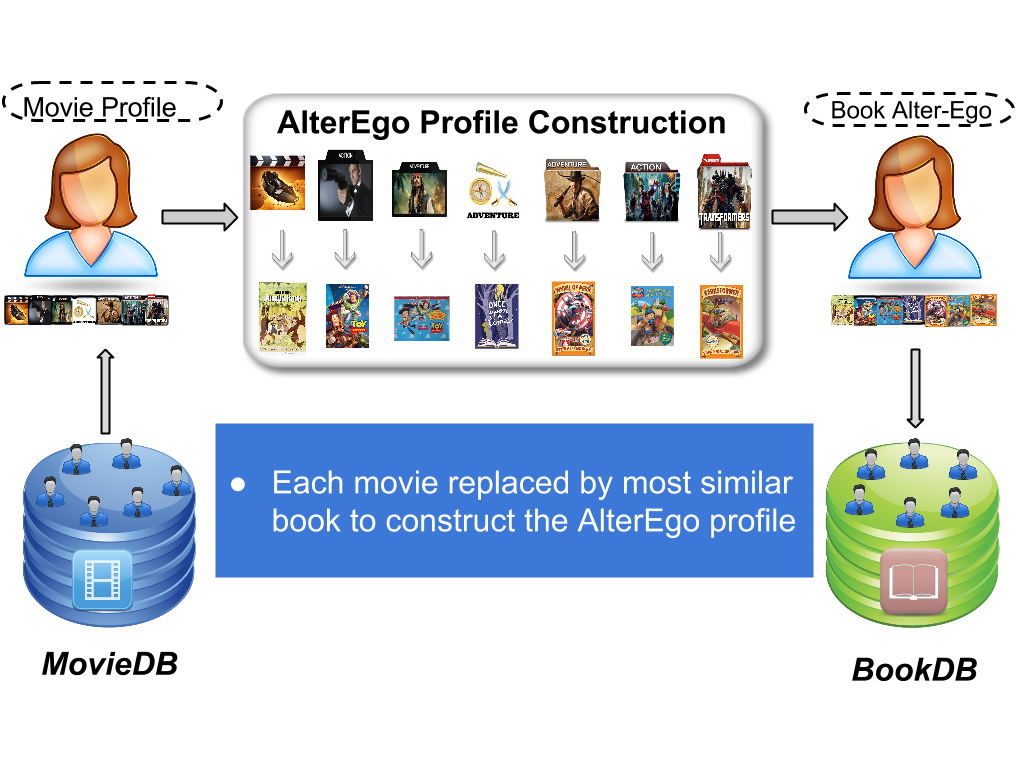
\includegraphics[height=2.5in,width=3.3in]{figures/AlterEgo.png}
\vspace{-12mm}
\caption{{\bf Alice's AlterEgo profile (in target domain) mapped from her original profile (in source domain).}}
\vspace{-2mm}
\label{fig:alterego}
\end{center}
\end{figure}

%\subsubsection*{{\it \large\crossrec} AlterEgo generation}

\noindent{\bf \crossrec AlterEgo generation.} The private mapping is performed in two steps which are as follows.

{\it Private replacement selection.} We consider Differential privacy~\cite{dwork2006calibrating} which is a technique for releasing statistical information about a database without revealing information about its individual entries. More specifically, differential privacy is defined as follows.


\begin{definition}[Differential Privacy~\cite{dwork2006calibrating}]
A randomized function $\mathcal{R}$ provides $\epsilon$-differential privacy if for all datasets $\mathcal{D}_1$ and $\mathcal{D}_2$, differing on at most one user profile, and all $t \in Range(\mathcal{R})$, the following inequality always holds:
$$\frac{Pr[\mathcal{R}(\mathcal{D}_{1} ) = t]}{Pr[\mathcal{R}(\mathcal{D}_{2}) = t]} \le exp(\epsilon)$$
\end{definition}


We leverage an exponential mechanism to design our differentially private replacement selection technique (Algorithm~\ref{Algo:prs}). The following theorem conveys our resulting privacy guarantee.

\begin{theorem}
Given an item $t_i$, the sensitivity of \graphsim is denoted by GS and the similarity between $t_i$ and any arbitrary item $t_j$ is denoted by $\graphsim(t_i,t_j)$. Then, the Private Replacement Selection (PRS) mechanism, which outputs $t_j$ as the replacement with a probability proportional to $exp(\frac{\epsilon \cdot \graphsim (t_i,t_j)}{2 \cdot GS})$, provides $\epsilon$-differential privacy.
\end{theorem}

\begin{proof}
Consider two datasets $D$ and $D'$ which differ at one user, say $u$. We denote the \graphsim($t_i$,$t_j$) in dataset D as $q(D,t_i,t_j)$ and $I(t_i)$ as the set of items in target domain with quantified \graphsim values. The global sensitivity (GS) is defined as $max_{D'}||q(D,t_i,t_j) - q(D',t_i,t_j)||_1$. Our PRS mechanism outputs an item $t_j$ as a private replacement for $t_i$. Then, we have the following:
\begin{flalign*}
 &
\frac{Pr[PRS(t_i, I(t_i), q(D,I(t_i)))= t_j]}{Pr[PRS(t_i, I(t_i), q(D',I(t_i)))= t_j]}& 
\end{flalign*}

\begin{flalign*}
 &= \frac{exp(\frac{\epsilon \cdot q(D,t_i,t_j)}{2 \cdot GS})}{\sum \limits_{t_k \in I(t_i)} exp(\frac{\epsilon \cdot q(D,t_i,t_k)}{2 \cdot GS})} \div \frac{exp(\frac{\epsilon \cdot q(D',t_i,t_j)}{2 \cdot GS})}{\sum \limits_{t_k \in I(t_i)} exp(\frac{\epsilon \cdot q(D',t_i,t_k)}{2 \cdot GS})} & 
\end{flalign*}


\begin{flalign*}
 &= \underbrace{\frac{exp(\frac{\epsilon \cdot q(D,t_i,t_j)}{2 \cdot GS})}{exp(\frac{\epsilon \cdot q(D',t_i,t_j)}{2 \cdot GS})}}_\text{P} \cdot \underbrace{\frac{\sum \limits_{t_k \in I(t_i)} exp(\frac{\epsilon \cdot q(D',t_i,t_k)}{2 \cdot GS})}{\sum \limits_{t_k \in I(t_i)} exp(\frac{\epsilon \cdot q(D,t_i,t_k)}{2 \cdot GS})}}_\text{Q}&
\end{flalign*}

\begin{flalign*}
&P= exp(\frac{\epsilon \cdot (q(D,t_i,t_j) -q(D',t_i,t_j))}{2 \cdot GS}) \le exp(\frac{\epsilon \cdot GS}{2 \cdot GS})= exp(\frac{\epsilon}{2})&
\end{flalign*}

\begin{flalign*}
&Q= \frac{\sum \limits_{t_k \in I(t_i)} exp(\frac{\epsilon \cdot q(D',t_i,t_k)}{2 \cdot GS})}{\sum \limits_{t_k \in I(t_i)} exp(\frac{\epsilon \cdot q(D,t_i,t_k)}{2 \cdot GS})} \le \frac{\sum \limits_{t_k \in I(t_i)} exp(\frac{\epsilon \cdot (q(D,t_i,t_k) +GS)}{2 \cdot GS})}{\sum \limits_{t_k \in I(t_i)} exp(\frac{\epsilon \cdot q(D,t_i,t_k)}{2 \cdot GS})}&
\end{flalign*}
\begin{flalign*}
&= \frac{ exp(\frac{\epsilon}{2}) \cdot \sum \limits_{t_k \in I(t_i)} exp(\frac{\epsilon \cdot q(D,t_i,t_k)}{2 \cdot GS})}{\sum \limits_{t_k \in I(t_i)} exp(\frac{\epsilon \cdot q(D,t_i,t_k)}{2 \cdot GS})} = exp(\frac{\epsilon}{2})&
\end{flalign*}

Therefore, we have:
$$
\frac{Pr[PRS(t_i, I(t_i), q(D,I(t_i)))= t_j]}{Pr[PRS(t_i, I(t_i), q(D',I(t_i)))= t_j]} \le exp(\epsilon)
$$
Hence, PRS provides $\epsilon$-differential privacy.
\end{proof}



%In~\cite{zhu2013differential,zhu2014effective}, the authors proposed a private neighbor selection mechanism which can provide high quality neighbors and gurantees differential privacy simultaneously. Inspired by this mechanism, we compute the private replacement for the actual item leveraging the exponential mechanism as shown in Algorithm~\ref{Algo:prs}.

\begin{algorithm}[!htb]
\caption{\small\itshape Private Replacement Selection : PRS($t_i$, I($t_i$), \emph{X-Sim}(I($t_i$))) where I($t_i$) is the set of items in the target domain with \graphsim values.}
\label{Algo:prs}
\begin{algorithmic}[1]
\Require $\epsilon, t_i, I(t_i), \emph{X-Sim}(I(t_i))$		\hfill $\rhd$ $\epsilon:$ Privacy parameter
\State Global sensitivity for \graphsim:\\ GS= $|\graphsim_{max} - \graphsim_{min}|$=2

\For  {item $t_j$ in $I(t_i)$}
\State Allocate probability as:
\vspace{-3mm}
$$
\frac{exp(\frac{\epsilon \cdot \graphsim (t_i,t_j)}{2 \cdot GS})}{\sum \limits_{t_k \in I(t_i)} exp(\frac{\epsilon \cdot \graphsim (t_i,t_k)}{2 \cdot GS})}
$$
\vspace{-4mm}
\EndFor


\State Sample an element $t$ from $I(t_i)$ according to their probability.
\State Return $t$; \hfill $\rhd$ $\epsilon$-differentially private replacement for $t_i$
\end{algorithmic}
\end{algorithm}


{\it AlterEgo profile construction.} In this step, we replace every item rated by Alice in $D^S$ with the item in $D^T$ returned by the private mechanism in the previous step. This item replacement leads to an AlterEgo profile of Alice in the target domain.

Note that this private AlterEgo profile protects the privacy of the straddlers, users who rated in both the domains, as the ratings of these users are used to compute the heterogeneous similarities leaving their privacy at risk~\cite{ramakrishnan2001privacy}. In addition, if the domains are typically two different applications owned by different companies like Netflix and Last.fm, then this mechanism aids the usage of AlterEgo profiles while preventing curious or malicious users to infer about the preferences of others. 



%Additionally, this privacy mechanism also facilitates the exchange of AlterEgo profiles without releasing private information about their customers. Note that there are ways to compute the heterogeneous cosine similarities using secure protocols based on zero-knowledge proofs~\cite{yang2013secure,kikuchi2010privacy,zhang2014secure,wong2013privacy} and the homogeneous item similarties can be released in a differential private manner~\cite{mcsherry2009differentially} but this is out of the scope of this paper.  



\subsection{Recommendation Phase}
We now present the recommendation computation steps. Again, we first explain the non-private case followed by the private one.

%\subsubsection*{{\it \large\npcrossrec} recommendation} leveraging the notion of \emph{temporal collaborative filtering}~\cite{liu2010online, ding2005time}
\noindent{\bf \npcrossrec recommendation.} The AlterEgo profile of Alice is used along with the original profiles in the target domain to compute the top-k similar users for Alice and then compute recommendations for Alice leveraging the profiles of the $k$ most similar users from the target domain using Algorithm \ref{ub_cf}. The item-based version of \crossrec leverages this AlterEgo profile and computes the recommendations as demonstrated in Algorithm \ref{ib_cf}. For the item-based version of \crossrec, we improve the recommendation quality further by adding a time-based weight to the ratings. The predictions (Equation~\ref{pred_ib_cf}), weighted by the time-based parameter ($\alpha$), for the ratings are computed as follows.
\begin{equation}
\label{pred_ib_cf_time}
Pred[i] (t)=\bar{r}_{i} +\frac{\sum_{j \in N_{i}} \tau(i,j) \cdot (r_{A,j}- \bar{r}_j) \cdot e^{-\alpha (t-t_{A,j})}}{\sum_{j \in N_{i}} |\tau(i,j)| \cdot e^{-\alpha (t-t_{A,j})} } 
\end{equation}
Note that the prediction has a time-based relevance factor ($e^{-\alpha (t-t_{A,j})}$) with decaying rate controlled by parameter $\alpha$ to determine each rating's weight for the prediction computation. Here, $t_{A,j}$ denotes the time when user $A$ rated item $j$.\footnote{This time unit is the index of the item in the user's profile ordered by the actual timestamp.} The time-based CF feature is applicable to the item-based CF approach as the prediction computation (Equation~\ref{pred_ib_cf_time}) for a user $A$ is dependent only on her previous ratings for similar items and thereby leverages time as observed by $A$.

%\subsubsection*{{\it \large\crossrec} recommendation}
\noindent{\bf \crossrec recommendation.} 
To demonstrate the flexibility of our heterogeneous recommender, the recommendation step is integrated with a differential private approach, inspired by Zhu et al.~\cite{zhu2013differential,zhu2014effective}, to protect against curious users. We implemented both item-based and user-based versions of \crossrec. The user-based recommendation mechanism is demonstrated in Algorithm~\ref{PrivRecoAlgo} which leverages the PNSA mechanism (Algorithm~\ref{Algo:pnsa}). Now, we present the correctness proof of our revised recommendation-aware sensitivity.\footnote{Our notion of recommendation-aware sensitivity is different from the one presented in~\cite{zhu2013differential,zhu2014effective}.}

\begin{definition}[Local Sensitivity]
For a given function $f: \mathcal{R} \rightarrow R$ and a dataset $D$, the Local Sensitivity of $f$ is defined as $LS_f = \max \limits_{D'}\Arrowvert f(D) - f(D')\Arrowvert_1$, where $D$ and $D'$ are neighboring datasets which differ at one user profile. 
\end{definition}


\begin{theorem}[Recommendation-aware sensitivity]
\begin{sloppypar}
Given a score function $q: \mathcal{R} \rightarrow R$ and a dataset $D$, we define the recommendation-aware sensitivity corresponding to a score function $q_i(I,t_j)$ for a pair of items $t_i$ and $t_j$ as:
\end{sloppypar}
\begin{flalign*}
&RS(t_i, t_j) = max \{ max_{u_x \in U_{ij}} (\frac{r_{t_{xi}} \times r_{t_{xj}}}{\parallel r'_{t_i} \parallel \times \parallel r'_{t_j} \parallel}),&
\end{flalign*}

\begin{flalign*}
& max_{u_x \in U_{ij}} (\frac{r_{t_i} \cdot r_{t_j}} {\parallel r'_{t_i} \parallel \times \parallel r'_{t_j} \parallel} - \frac{r_{t_i} \cdot r_{t_j}} {\parallel r_{t_i} \parallel \times \parallel r_{t_j} \parallel})\} &
\end{flalign*}
\end{theorem}




\begin{proof}
Now, we provide the proof of the recommendation-aware sensitivity. First, we have:
\begin{align*}
RS(t_i, t_j) &= 
max \parallel s(t_i, t_j) - s'(t_i, t_j)\parallel_1
\end{align*}

Next, we insert the similarity values for $s(t_i, t_j)$. A rating vector $r_{t_i} = \lbrack r_{t_{ai}}, ..., r_{t_{xi}}, r_{t_{yi}} \rbrack$ consists of all the ratings for an item $t_i$. Note that here a rating $r_{t_{xi}}$ denotes the result after subtracting the average rating of user $x$ ($\bar{r_x}$) from the actual rating provide by $x$ for an item $i$. Now, we have:
\begin{flalign*}
& s(t_i, t_j) - s'(t_i, t_j) = \frac{r_{t_i} \cdot r_{t_j}}{\parallel r_{t_i} \parallel \times \parallel r_{t_j} \parallel} - 
\frac{r'_{t_i} \cdot r'_{t_j}}{\parallel r'_{t_i} \parallel \times \parallel r'_{t_j} \parallel} &
\end{flalign*}

\begin{flalign*}
& =\frac{r_{t_i} \cdot r_{t_j} \times \parallel r'_{t_i} \parallel \times \parallel r'_{t_j} \parallel -
r'_{t_i} \cdot r'_{t_j} \times \parallel r_{t_i} \parallel \times \parallel r_{t_j} \parallel 
}{\parallel r_{t_i} \parallel \times \parallel r_{t_j} \parallel \times \parallel r'_{t_i} \parallel \times \parallel r'_{t_j} \parallel}=\frac{P}{Q} &
\end{flalign*}

Now, we assume that the profile of a user $x$, in $D$, is not present in $D'$. This user rated both $t_i$ and $t_j$. Note that if this user rated one of these items or none, then the similarity value does not depend on the presence or absence of this user in the dataset. Hence, we have: $\parallel r'_{t_i} \parallel \times \parallel r'_{t_j} \parallel \leq \parallel r_{t_i} \parallel \times \parallel r_{t_j} \parallel$. 

Now, we have P= ($r_{t_i} \cdot r_{t_j} \times \parallel r'_{t_i} \parallel \times \parallel r'_{t_j} \parallel -
r'_{t_i} \cdot r'_{t_j} \times \parallel r_{t_i} \parallel \times \parallel r_{t_j} \parallel$) and Q=($\parallel r_{t_i} \parallel \times \parallel r_{t_j} \parallel \times \parallel r'_{t_i} \parallel \times \parallel r'_{t_j} \parallel$).
Hence, $Q \geq 0$ and depending on whether $P \geq 0$ or $P \leq 0$ we have two conditions which are as follows.

If $P \geq 0$, then we have:
\begin{flalign*}
&\parallel s(t_i, t_j) - s'(t_i, t_j) \parallel_1&
\end{flalign*}

\begin{flalign*}
&=\frac{r_{t_i} \cdot r_{t_j} \times \parallel r'_{t_i} \parallel \times \parallel r'_{t_j} \parallel -
r'_{t_i} \cdot r'_{t_j} \times \parallel r_{t_i} \parallel \times \parallel r_{t_j} \parallel 
}{\parallel r_{t_i} \parallel \times \parallel r_{t_j} \parallel \times \parallel r'_{t_i} \parallel \times \parallel r'_{t_j} \parallel} &
\end{flalign*}

\begin{flalign*}
& \leq \frac{(r_{t_i} \cdot r_{t_j} - r'_{t_i} \cdot r'_{t_j}) \times \parallel r_{t_i} \parallel \times \parallel r_{t_j} \parallel}
{\parallel r_{t_i} \parallel \times \parallel r_{t_j} \parallel \times \parallel r'_{t_i} \parallel \times \parallel r'_{t_j} \parallel} &
\end{flalign*}

\begin{flalign*}
&= \frac{(r_{t_i} \cdot r_{t_j} - r'_{t_i} \cdot r'_{t_j})}
{\parallel r'_{t_i} \parallel \times \parallel r'_{t_j} \parallel}&
\end{flalign*}

If $P \leq 0$, then we have:
\begin{flalign*}
& \parallel s(t_i, t_j) - s'(t_i, t_j) \parallel_1 &
\end{flalign*}

\begin{flalign*}
&=
\frac{r'_{t_i} \cdot r'_{t_j} \times \parallel r_{t_i} \parallel \times \parallel r_{t_j} \parallel - r_{t_i} \cdot r_{t_j} \times \parallel r'_{t_i} \parallel \times \parallel r'_{t_j} \parallel }
{\parallel r_{t_i} \parallel \times \parallel r_{t_j} \parallel \times \parallel r'_{t_i} \parallel \times \parallel r'_{t_j} \parallel} &
\end{flalign*}

\begin{flalign*}
& = \frac{(r_{t_i} \cdot r_{t_j} - r_{t_{xi}} \times r_{t_{xj}}) \times \parallel r_{t_i} \parallel \times \parallel r_{t_j} \parallel}
{\parallel r_{t_i} \parallel \times \parallel r_{t_j} \parallel \times \parallel r'_{t_i} \parallel \times \parallel r'_{t_j} \parallel} &
\end{flalign*}

\begin{align*}
& - \frac{r_{t_i} \cdot r_{t_j} \times \parallel r'_{t_i} \parallel \times \parallel r'_{t_j} \parallel}{\parallel r_{t_i} \parallel \times \parallel r_{t_j} \parallel \times \parallel r'_{t_i} \parallel \times \parallel r'_{t_j} \parallel} &
\end{align*}

\begin{flalign*}
&= \frac{r_{t_i} \cdot r_{t_j} \times (\parallel r_{t_i} \parallel \times \parallel r_{t_j} \parallel  - \parallel r'_{t_i} \parallel \times \parallel r'_{t_j} \parallel)}
{\parallel r_{t_i} \parallel \times \parallel r_{t_j} \parallel \times \parallel r'_{t_i} \parallel \times \parallel r'_{t_j} \parallel}  &
\end{flalign*}


\begin{align*}
& - \frac{r_{t_{xi}} \times r_{t_{xj}} \times \parallel r_{t_i} \parallel \times \parallel r_{t_j} \parallel}{\parallel r_{t_i} \parallel \times \parallel r_{t_j} \parallel \times \parallel r'_{t_i} \parallel \times \parallel r'_{t_j} \parallel}&
\end{align*}

\begin{flalign*}
& \leq \frac{r_{t_i} \cdot r_{t_j} \times (\parallel r_{t_i} \parallel \times \parallel r_{t_j} \parallel  - \parallel r'_{t_i} \parallel \times \parallel r'_{t_j} \parallel)}
{\parallel r_{t_i} \parallel \times \parallel r_{t_j} \parallel \times \parallel r'_{t_i} \parallel \times \parallel r'_{t_j} \parallel}&
\end{flalign*}

\begin{flalign*}
&=\frac{r_{t_i} \cdot r_{t_j}} {\parallel r'_{t_i} \parallel \times \parallel r'_{t_j} \parallel} - \frac{r_{t_i} \cdot r_{t_j}} {\parallel r_{t_i} \parallel \times \parallel r_{t_j} \parallel}&
\end{flalign*}

Hence, we have the recommendation-aware sensitivity as:
\begin{flalign*}
&RS(t_i, t_j) = max \{ max_{u_x \in U_{ij}} (\frac{r_{t_{xi}} \times r_{t_{xj}}}{\parallel r'_{t_i} \parallel \times \parallel r'_{t_j} \parallel}),&
\end{flalign*}

\begin{flalign*}
& max_{u_x \in U_{ij}} (\frac{r_{t_i} \cdot r_{t_j}} {\parallel r'_{t_i} \parallel \times \parallel r'_{t_j} \parallel} - \frac{r_{t_i} \cdot r_{t_j}} {\parallel r_{t_i} \parallel \times \parallel r_{t_j} \parallel})\} &
\end{flalign*}
\end{proof}



%(Our correctness proof is available in~\autoref{sensitivity}). 
%In the following, we revisit the two theorems, presented in~\cite{zhu2013differential,zhu2014effective}, which prove that this truncated similarity can enhance the quality of neighbors.
We use a \emph{truncated similarity} (Step 5 in Algorithm~\ref{Algo:pnsa}) along with our revised recommendation-aware sensitivity to enhance the quality of selected neighbors. Now, we present two theorems which prove that this truncated similarity along with our recommendation-aware sensitivity can enhance the quality of neighbors. The proofs have been omitted due to lack of space.\footnote{Our proofs are presented in our companion technical report for interested readers~\cite{}.}


% and follow the same methodology as in~\cite{zhu2013differential,zhu2014effective}

\begin{theorem}
\label{theorem_1}
Given an item $t_i$, we denote its $k$ neighbors by $N_k(t_i)$, the maximal length of all the rating vector pairs by $|v|$ and the recommendation-aware sensitivity between $t_i$ and other items by RS. Then, for a small constant  $0< \rho <1$, the similarity of all the items in $N_k(t_i)$ are larger than $(Sim_k -w)$ with a probability at least $1 - \rho$, where $w=min(Sim_k(I(t_i)), \frac{4k \times RS}{\epsilon'} \times ln\frac{k \times (|v| - k)}{\rho})$ and $Sim_k$ is the minimal similarity among the items in $N_k(t_i)$.
\end{theorem}

Intuitively, Theorem~\ref{theorem_1} implies that the selected neighbors have similarities greater than some threshold value $(Sim_k -w)$ with a high probability.

\begin{theorem}
\label{theorem_2}
Given an item $t_i$, for a small constant   $0 <\rho <1$, all items with similarities greater than $(Sim_k +w)$ are present in $N_k(t_i)$ with a probability at least $1-\rho$ where $w=min(Sim_k(I(t_i)), \frac{4k \times RS}{\epsilon'} \times ln\frac{k \times (|v| - k)}{\rho})$.
\end{theorem}

Intuitively, Theorem~\ref{theorem_2} implies that the items with similarities greater than some threshold value $(Sim_k +w)$ are selected as neighbors with a high probability.

Both theorems prove that the truncated similarity along with our recommendation-aware sensitivity provide good quality of neighbors while providing $\epsilon'/2$-differential privacy. The predictions are finally computed leveraging the PNCF mechanism (Algorithm~\ref{PrivRecoAlgo}) which adds Laplacian noise to provide $\epsilon'/2$-differential privacy. By additive property of differential privacy, PNSA and PNCF together provides $\epsilon'$-differential privacy.

The item-based version of \crossrec includes the additional feature of \emph{time-based relevant} predictions to boost the recommendation quality traded for privacy.



\begin{algorithm}[!htb]
\caption{\small\itshape Private Neighbor Selection Algorithm : PNSA($t_i$, I($t_i$), \emph{Sim}(I($t_i$)), k) where I($t_i$) is the set of items with pre-computed similarity values.}
\label{Algo:pnsa}
\begin{algorithmic}[1]
\Require $\epsilon', w, t_i, I(t_i), \emph{Sim}(I(t_i))$, k		\hfill $\rhd$ $\epsilon':$ Privacy 
    \State $C_1 = \lbrack t_j | s(t_i, t_j) \geq \emph{Sim}_k(I(t_i))-w, t_j \in I(t_i)\rbrack$
    \State $C_0 = \lbrack t_j | s(t_i, t_j) < \emph{Sim}_k(I(t_i))-w, t_j \in I(t_i)\rbrack$
    \State $w=min(\emph{Sim}_k(I(t_i)), \frac{4k \times RS}{\epsilon'} \times ln\frac{k \times (|v| - k)}{\rho})$
\State Recommendation-aware sensitivity for ($t_i,t_j$): RS($t_i$,$t_j$)
\vspace{-3mm}
{\small
\begin{flalign*}
{\bf RS(t_i, t_j) }= max \{
max_{u_x \in U_{ij}} (\frac{r_{t_{xi}} \times r_{t_{xj}}}{\parallel r'_{t_i} \parallel \times \parallel r'_{t_j} \parallel}),&\\ 
 max_{u_x \in U_{ij}} (\frac{r_{t_i} \cdot r_{t_j}} {\parallel r'_{t_i} \parallel \times \parallel r'_{t_j} \parallel} - \frac{r_{t_i} \cdot r_{t_j}} {\parallel r_{t_i} \parallel \times \parallel r_{t_j} \parallel)}
)\}
\end{flalign*}}
\vspace{-4mm}
    \State $\widehat{\emph{Sim}} = max(\emph{Sim}(t_i, t_j), \emph{Sim}_k(I(t_i)) - w)$
	\For  {N=1:k}
   \For  {item $t_j$ in $I(t_i)$}
    \State Allocate probability as:
    \vspace{-3mm}
    $$
    \frac{exp(\frac{\epsilon' \cdot \widehat{\emph{Sim}}(t_i, t_j)}{4 \times  k \times RS(t_i, t_j)})}{\sum \limits_{l \in C_1} exp(\frac{\epsilon' \cdot \widehat{\emph{Sim}}(t_i, t_l)}{4 \times k \times RS(t_i, t_l)}) +  \sum \limits_{l \in C_0} exp(\frac{\epsilon' \cdot \widehat{\emph{Sim}}(t_i, t_l)}{4 \times k \times RS(t_i, t_l)})}
	$$
    \vspace{-4mm}
	\EndFor 

	\State Sample an element $t$ from $C_1$ and $C_0$ without replacement according to their probability.
	\State $N_k(t_i)=N_k(t_i) \cup t$
	\EndFor
	\State Return $N_k(t_i)$; 
\end{algorithmic}
\end{algorithm}


\begin{algorithm}[!htb]
\caption{\small\itshape Private Recommendation: PNCF($P_A, N_A, \mathcal{I}$): $P_A$ denotes the AlterEgo profile of Alice, $N_A$ denotes private neighbors of Alice from PSA mechanism and $I$ denotes the set of all items.}
\label{PrivRecoAlgo}
\begin{algorithmic}[1]
\State var Pred[]; \hfill $\rhd$ Predictions for Alice
\State var $\bar{r}$; \hfill $\rhd$ Average rating for each user
\For {$C$ : $user$ in $N_A$}
\State $\tau_{n}(A, C) = \tau(A, C) + Lap(\frac{RS(A, C)}{\epsilon' / 2});$\hfill $\rhd \epsilon':$ Privacy
\EndFor
\For {$i$ : $item$ in $I$}
\State $Pred[i]=\bar{r}_{A} +\frac{\sum_{B \in N_{A}} \tau_{n}(A,B) \cdot (r_{B,i}- \bar{r}_B)}{\sum_{B \in N_{A}} |\tau_{n}(A,B)| } ;$
\EndFor
\State $R_{A}=subList(N,sort(Pred));$
\State \textbf{return:} $R_{A}$; \hfill $\rhd$ Top-N recommendations for Alice
\end{algorithmic}
\end{algorithm}
